%%%%%%%%%%%%%%%%%%%%%%%%%%%%%%%%%%%%%%%%%%%%%%%%%%%%%%%%%%%%%%%%%%%%%%%%%%%%%%%%
\documentclass[letterpaper, 10 pt, conference]{ieeeconf}  % Comment this line out
                                                          % if you need a4paper
                                                          
%\documentclass[a4paper, 10pt, conference]{ieeeconf}      % Use this line for a4
                                                          % paper
                                                          
\IEEEoverridecommandlockouts                              % This command is only
                                                          % needed if you want to
                                                          % use the \thanks command
\overrideIEEEmargins
% See the \addtolength command later in the file to balance the column lengths
% on the last page of the document
%%%%%%%%%%%%%%%%%%% PACKAGES %%%%%%%%%%%%%%%%%%%%%%%%%%%%%%%%%%%%%%%%%%
% The following packages can be found on http:\\www.ctan.org
\usepackage{graphics} % for pdf, bitmapped graphics files
%\usepackage{epsfig} % for postscript graphics files
%\usepackage{mathptmx} % assumes new font selection scheme installed
%\usepackage{times} % assumes new font selection scheme installed
\usepackage{amsmath} % assumes amsmath package installed
%\usepackage{amssymb}  % assumes amsmath package installed
\usepackage{graphicx}
%%%%%%%%%%%%%%%%%%%%%%%%%%%%%%%%%%%%%%%%%%%%%%%%%%%%%%%%%%%%%%%%%%%%%%

\title{\LARGE \bf
Writing a document in \LaTeX
}

% This is where you will enter your name and affiliation!
\author{Dr. Trevor Michael Tomesh\\
University of Regina - Computer Science\\
email: trevor.tomesh@uregina.ca
}

\begin{document}

\maketitle
\thispagestyle{empty}
\pagestyle{empty}


%%%%%%%%%%%%%%%%%%%%%%%%%%%%%%%%%%%%%%%%%%%%%%%%%%%%%%%%%%%%%%%%%%%%%%%%%%%%%%%%
\begin{abstract}
In this paper, I am demonstrating to my students how to write a well 
formatted paper in the \LaTeX\ typesetting language. We will cover a few
key features of the language. 
\end{abstract}
%%%%%%%%%%%%%%%%%%%%%%%%%%%%%%%%%%%%%%%%%%%%%%%%%%%%%%%%%%%%%%%%%%%%%%%%%%%%%%%%

\keywords{ -one, two, three, four}



\section{SUMMARY}
This document just shows some of the basic cool things that you can do in \LaTeX. 
It can be used as a template to write your own well formatted IEEE style papers. 
\LaTeX\ is an important step in getting a paper published in a respectable journal 
and it is therefore very important to learn it.

%%%%%%%%%%%%%%%%%%%%%%%%%%%%%%%%%%%%%%%%%%%%%%%%%%%%%%%%%%%%%%%%%%%%%%%%%%%%%%%%%

\section{HOW TO CITE THINGS}
A key part of writing an academic paper is being able to cite things properly. This is how you 
cite a source \cite{c1} in \LaTeX\ using the IEEE standard. If you want to quote someone, you need to do something like the following. According to Chen, ``this is kind of a pain in the butt \cite{c2}.'' The in-line citation should go as closely as possible to where the information that is being cited is present. According to G.O. Young, ``stuff be whack, yo \cite{c1}.''

%%%%%%%%%%%%%%%%%%%%%%%%%%%%%%%%%%%%%%%%%%%%%%%%%%%%%%%%%%%%%%%%%%%%%%%%%%%%%%%%%%

\section{MAKING A LIST}

There are a few different ways that you can make nice looking formatted lists
in \LaTeX. The following is an example of an ``enumerated'' list:

% uncomment this if you want to use 1.1, 1.2, etc.
% \renewcommand{\labelenumii}{\theenumii}
% \renewcommand{\theenumii}{\theenumi.\arabic{enumii}.}

\begin{enumerate}
    \item{This is the first item in my list}
    \begin{enumerate}
        \item{This is a sub-enumeration}
        \item{Here's another one!}
    \end{enumerate}
    \item{This is the second item in my list}
    \item{This is the third item in my list}
\end{enumerate}

Note that an enumerated list is a list that has numbers out in front of it!
You don't always need numbers, though. What if you want just a bunch of dots or something?
Well, we have a solution!

\begin{itemize}
    \item{This is the first thingy}
    \item{This is the second thingy}
    \item{another thingy}
    \begin{itemize}
        \item{A sub-thingy!}
        \item{Would ya look at that?!?}
    \end{itemize}
    \item{The last item in this list}
\end{itemize}

%%%%%%%%%%%%%%%%%%%%%%%%%%%%%%%%%%%%%%%%%%%%%%%%%%%%%

\section{FUN WITH SUBSECTIONS}

Sometimes, you have a section that you might want to 
divide into sub-sections. For example, the body of your paper
will probably need to be divided up into sub-sections. 
This is pretty straight-forward to do!

\subsection{Equations}

The equations are an exception to the prescribed specifications of this template. You will need to determine whether or not your equation should be typed using either the Times New Roman or the Symbol font (please no other font). To create multileveled equations, it may be necessary to treat the equation as a graphic and insert it into the text after your paper is styled. Number equations consecutively. Equation numbers, within parentheses, are to position flush right, as in (1), using a right tab stop. To make your equations more compact, you may use the solidus ( / ), the exp function, or appropriate exponents. Italicize Roman symbols for quantities and variables, but not Greek symbols. Use a long dash rather than a hyphen for a minus sign. Punctuate equations with commas or periods when they are part of a sentence, as in

$$
\alpha + \beta = \chi \eqno{(1)}
$$

If you would like to do an in-line equation, that's easy. You just $\alpha + \beta = \chi$. This is useful when you want to explain what individual symbols represent. The symbol $\alpha$, for example, is the first letter of the Greek alphabet. Hence the name ``alpha''. 

You can also have multiple equations that are numbered! For example, here is the Pythagorean Theorem:

$$
a^2 + b^2 = c^2 \eqno{(2)}
$$

You can write complex mathematical equations in \LaTeX\ quite easily! 

$$
 \iiint_V \mu(u,v) \,du\,dv \eqno{(3)}
$$


\section{USING THE TEMPLATE}

Use this sample document as your LaTeX source file to create your document. Save this file as {\bf root.tex}. You have to make sure to use the cls file that came with this distribution. If you use a different style file, you cannot expect to get required margins. Note also that when you are creating your out PDF file, the source file is only part of the equation. {\it Your \TeX\ $\rightarrow$ PDF filter determines the output file size. Even if you make all the specifications to output a letter file in the source - if you filter is set to produce A4, you will only get A4 output. }

It is impossible to account for all possible situation, one would encounter using \TeX. If you are using multiple \TeX\ files you must make sure that the ``MAIN`` source file is called root.tex - this is particularly important if your conference is using PaperPlaza's built in \TeX\ to PDF conversion tool.

\subsection{Headings, etc}

Text heads organize the topics on a relational, hierarchical basis. For example, the paper title is the primary text head because all subsequent material relates and elaborates on this one topic. If there are two or more sub-topics, the next level head (uppercase Roman numerals) should be used and, conversely, if there are not at least two sub-topics, then no subheads should be introduced. Styles named Heading 1, Heading 2, Heading 3, and Heading 4 are prescribed.

\subsection{Figures and Tables}

Positioning Figures and Tables: Place figures and tables at the top and bottom of columns. Avoid placing them in the middle of columns. Large figures and tables may span across both columns. Figure captions should be below the figures; table heads should appear above the tables. Insert figures and tables after they are cited in the text. Use the abbreviation Fig. 1, even at the beginning of a sentence.

\begin{table}[]
\centering
\begin{tabular}{|l|l|l|l|l|}
\hline
1 & 2 & 3 & 4 & 6 \\ \hline
2 & 3 & 4 & 5 & $\alpha$ \\ \hline
1 & 3 & 6 & 1 & 1.3 \\ \hline
1 & 2 & 5 & 6 &  $\pi$ \\ \hline
\end{tabular}
\caption{This is a table thingie.}
\end{table}

\begin{figure}[htp]
\centering
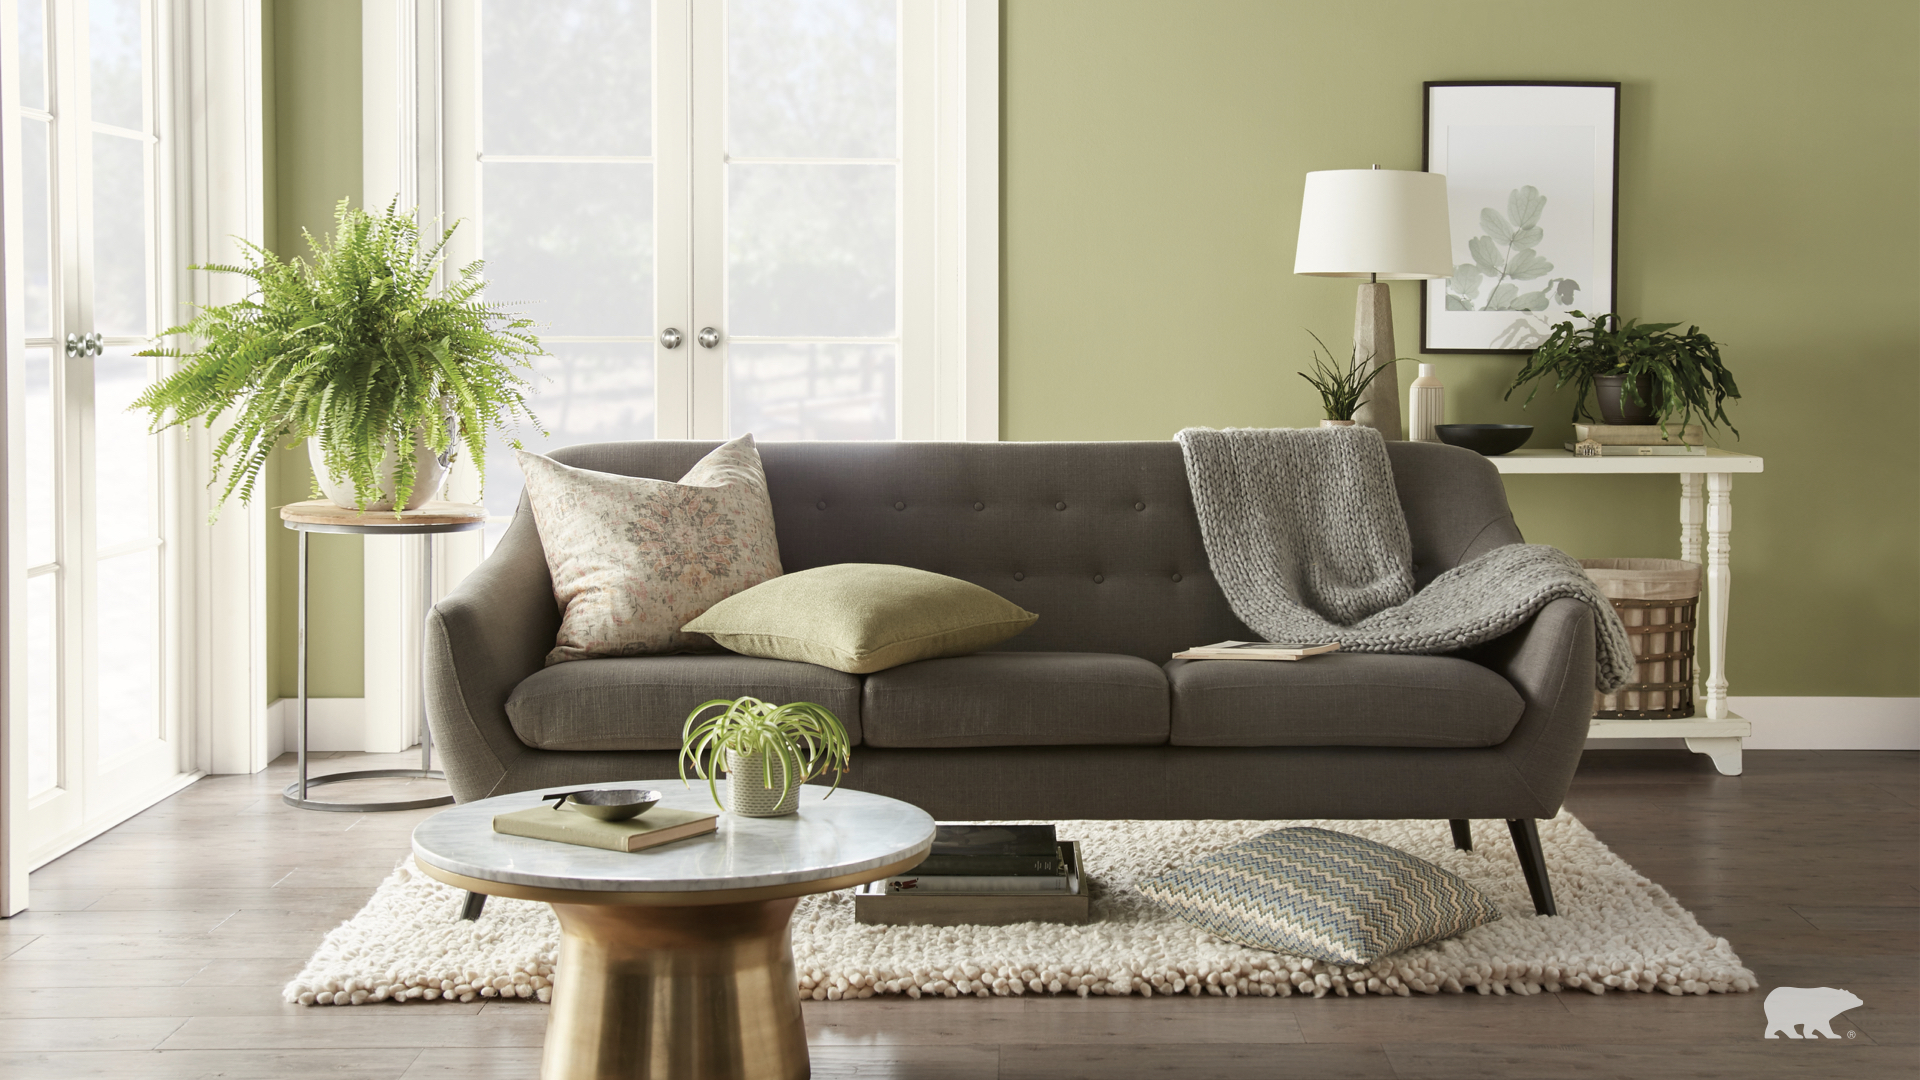
\includegraphics[width=4cm]{livingroom.jpeg}
\caption{This is a picture of a living room.}
\label{fig:livingroom}
\end{figure}  
   
 Look at Fig. ~\ref{fig:livingroom}! That's an awesome picture! As a rule of thumb, 
 you should \emph{never} have an image that you do not refer to in your text. Otherwise
 that is a waste of space. 

Figure Labels: Use 8 point Times New Roman for Figure labels. Use words rather than symbols or abbreviations when writing Figure axis labels to avoid confusing the reader. As an example, write the quantity Magnetization, or Magnetization, M, not just M. If including units in the label, present them within parentheses. Do not label axes only with units. In the example, write Magnetization (A/m) or Magnetization {A[m(1)]}, not just A/m. Do not label axes with a ratio of quantities and units. For example, write Temperature (K), not Temperature/K.

\section{CONCLUSION}
A great conclusion would be an end to my sweet suffering. ;-)

\addtolength{\textheight}{-12cm}   % This command serves to balance the column lengths
                                  % on the last page of the document manually. It shortens
                                  % the textheight of the last page by a suitable amount.
                                  % This command does not take effect until the next page
                                  % so it should come on the page before the last. Make
                                  % sure that you do not shorten the textheight too much.

%%%%%%%%%%%%%%%%%%%%%%%%%%%%%%%%%%%%%%%%%%%%%%%%%%%%%%%%%%%%%%%%%%%%%%%%%%%%%%%%



%%%%%%%%%%%%%%%%%%%%%%%%%%%%%%%%%%%%%%%%%%%%%%%%%%%%%%%%%%%%%%%%%%%%%%%%%%%%%%%%



%%%%%%%%%%%%%%%%%%%%%%%%%%%%%%%%%%%%%%%%%%%%%%%%%%%%%%%%%%%%%%%%%%%%%%%%%%%%%%%%
\section*{APPENDIX}

Appendixes should appear before the acknowledgment.

\section*{ACKNOWLEDGMENT}

The preferred spelling of the word acknowledgment in America is without an e after the g. Avoid the stilted expression, One of us (R. B. G.) thanks . . .  Instead, try R. B. G. thanks. Put sponsor acknowledgments in the unnumbered footnote on the first page.



%%%%%%%%%%%%%%%%%%%%%%%%%%%%%%%%%%%%%%%%%%%%%%%%%%%%%%%%%%%%%%%%%%%%%%%%%%%%%%%%

References are important to the reader; therefore, each citation must be complete and correct. If at all possible, references should be commonly available publications.

% if you want to break out of two column format for a little bit
% that is possible:
\onecolumn
\begin{figure}[htp]
\centering
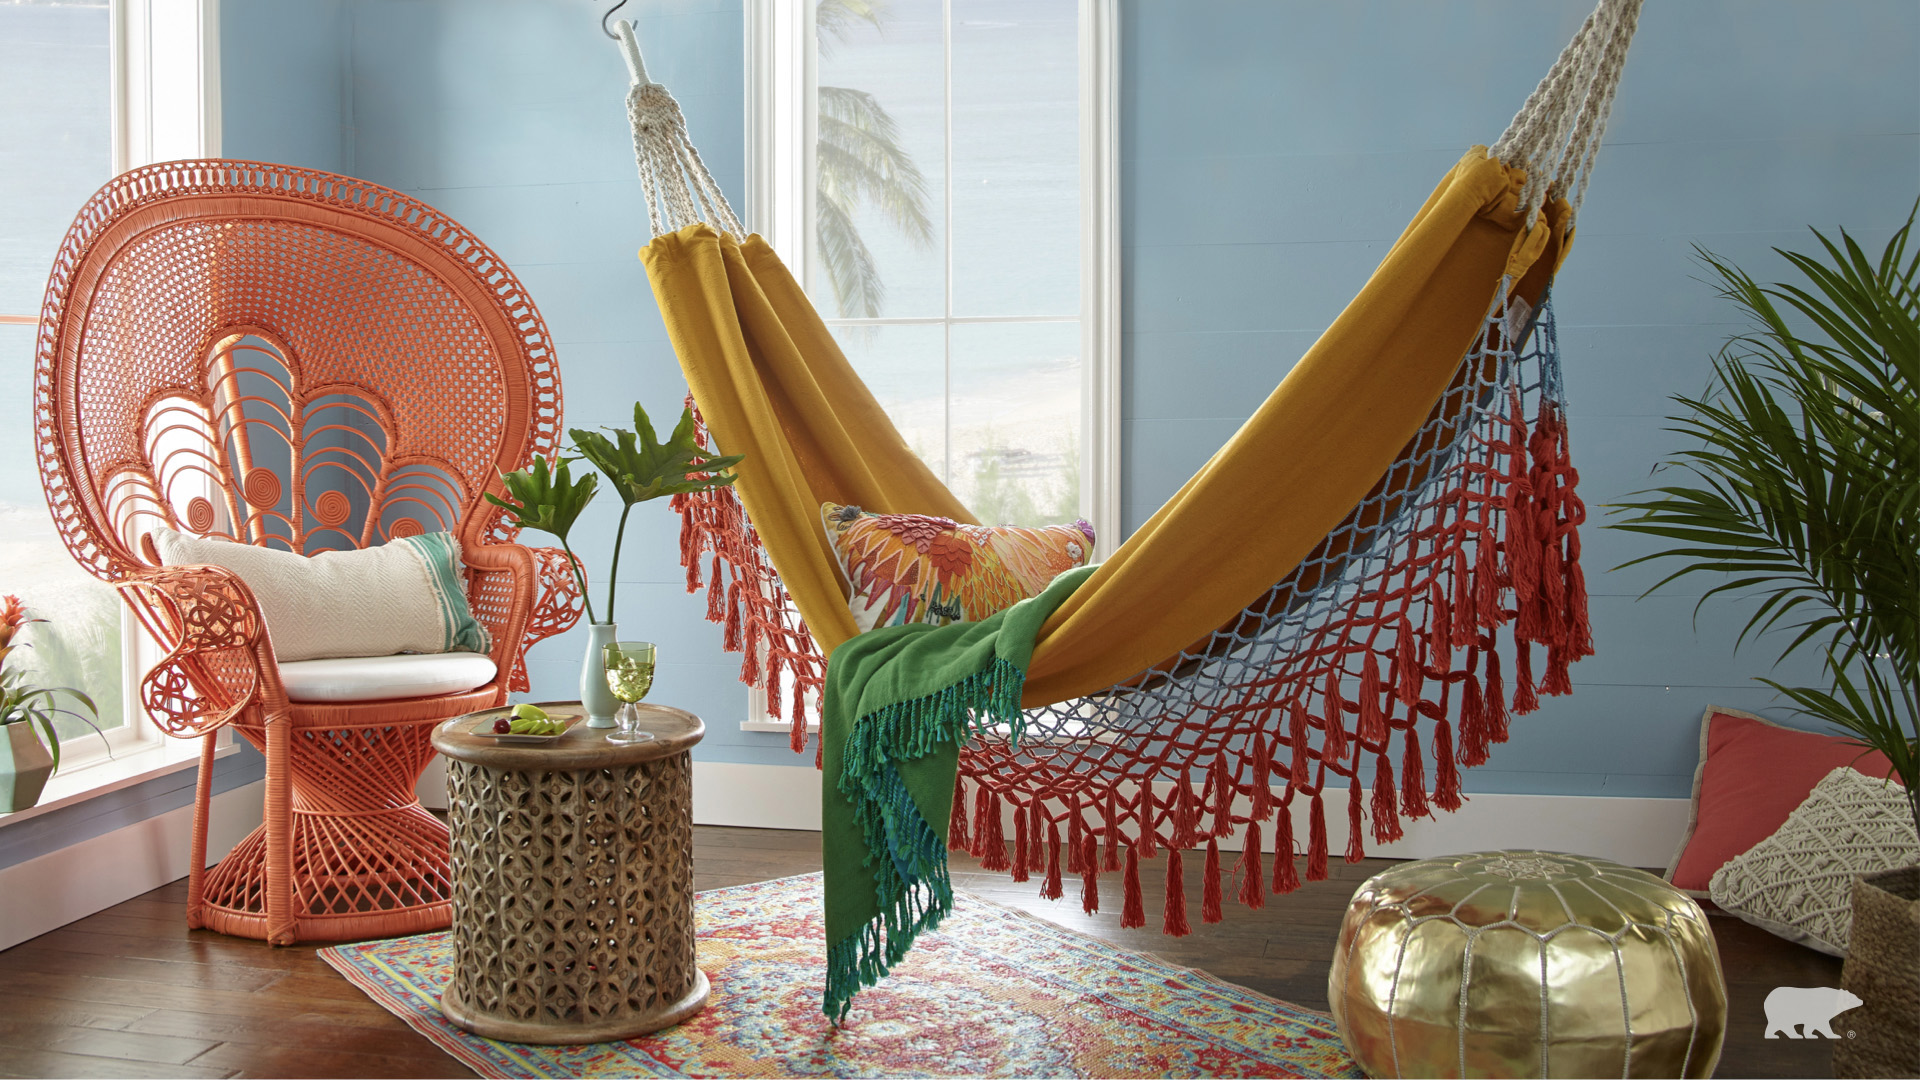
\includegraphics[width=10cm]{sunroom.jpeg}
\caption{This is a sunroom.}
\label{fig:sunroom}
\end{figure}
\twocolumn

\begin{thebibliography}{99}

\bibitem{c1} G. O. Young, Synthetic structure of industrial plastics (Book style with paper title and editor), 	in Plastics, 2nd ed. vol. 3, J. Peters, Ed.  New York: McGraw-Hill, 1964, pp. 15  64.
\bibitem{c2} W.-K. Chen, Linear Networks and Systems (Book style).	Belmont, CA: Wadsworth, 1993, pp. 123  135.
\bibitem{c3} H. Poor, An Introduction to Signal Detection and Estimation.   New York: Springer-Verlag, 1985, ch. 4.
\bibitem{c4} B. Smith, An approach to graphs of linear forms (Unpublished work style), unpublished.
\bibitem{c5} E. H. Miller, A note on reflector arrays (Periodical style Accepted for publication), IEEE Trans. Antennas Propagat., to be publised.
\bibitem{c6} J. Wang, Fundamentals of erbium-doped fiber amplifiers arrays (Periodical style Submitted for publication), IEEE J. Quantum Electron., submitted for publication.
\bibitem{c7} C. J. Kaufman, Rocky Mountain Research Lab., Boulder, CO, private communication, May 1995.
\bibitem{c8} Y. Yorozu, M. Hirano, K. Oka, and Y. Tagawa, Electron spectroscopy studies on magneto-optical media and plastic substrate interfaces(Translation Journals style), IEEE Transl. J. Magn.Jpn., vol. 2, Aug. 1987, pp. 740  741 [Dig. 9th Annu. Conf. Magnetics Japan, 1982, p. 301].
\bibitem{c9} M. Young, The Techincal Writers Handbook.  Mill Valley, CA: University Science, 1989.
\bibitem{c10} J. U. Duncombe, Infrared navigation Part I: An assessment of feasibility (Periodical style), IEEE Trans. Electron Devices, vol. ED-11, pp. 34  39, Jan. 1959.
\bibitem{c11} S. Chen, B. Mulgrew, and P. M. Grant, A clustering technique for digital communications channel equalization using radial basis function networks, IEEE Trans. Neural Networks, vol. 4, pp. 570  578, July 1993.
\bibitem{c12} R. W. Lucky, Automatic equalization for digital communication, Bell Syst. Tech. J., vol. 44, no. 4, pp. 547  588, Apr. 1965.
\bibitem{c13} S. P. Bingulac, On the compatibility of adaptive controllers (Published Conference Proceedings style), in Proc. 4th Annu. Allerton Conf. Circuits and Systems Theory, New York, 1994, pp. 8  16.
\bibitem{c14} G. R. Faulhaber, Design of service systems with priority reservation, in Conf. Rec. 1995 IEEE Int. Conf. Communications, pp. 3  8.
\bibitem{c15} W. D. Doyle, Magnetization reversal in films with biaxial anisotropy, in 1987 Proc. INTERMAG Conf., pp. 2.2-1  2.2-6.
\bibitem{c16} G. W. Juette and L. E. Zeffanella, Radio noise currents n short sections on bundle conductors (Presented Conference Paper style), presented at the IEEE Summer power Meeting, Dallas, TX, June 22  27, 1990, Paper 90 SM 690-0 PWRS.
\bibitem{c17} J. G. Kreifeldt, An analysis of surface-detected EMG as an amplitude-modulated noise, presented at the 1989 Int. Conf. Medicine and Biological Engineering, Chicago, IL.
\bibitem{c18} J. Williams, Narrow-band analyzer (Thesis or Dissertation style), Ph.D. dissertation, Dept. Elect. Eng., Harvard Univ., Cambridge, MA, 1993. 
\bibitem{c19} N. Kawasaki, Parametric study of thermal and chemical nonequilibrium nozzle flow, M.S. thesis, Dept. Electron. Eng., Osaka Univ., Osaka, Japan, 1993.
\bibitem{c20} J. P. Wilkinson, Nonlinear resonant circuit devices (Patent style), U.S. Patent 3 624 12, July 16, 1990. 


\end{thebibliography}

\end{document}
